\documentclass[a4paper,11pt,landscape]{article}
\usepackage{amsmath}
\usepackage{amsfonts}
\usepackage{tikz}
\usetikzlibrary{matrix,shapes,arrows,positioning,chains, calc}
\begin{document}
	
	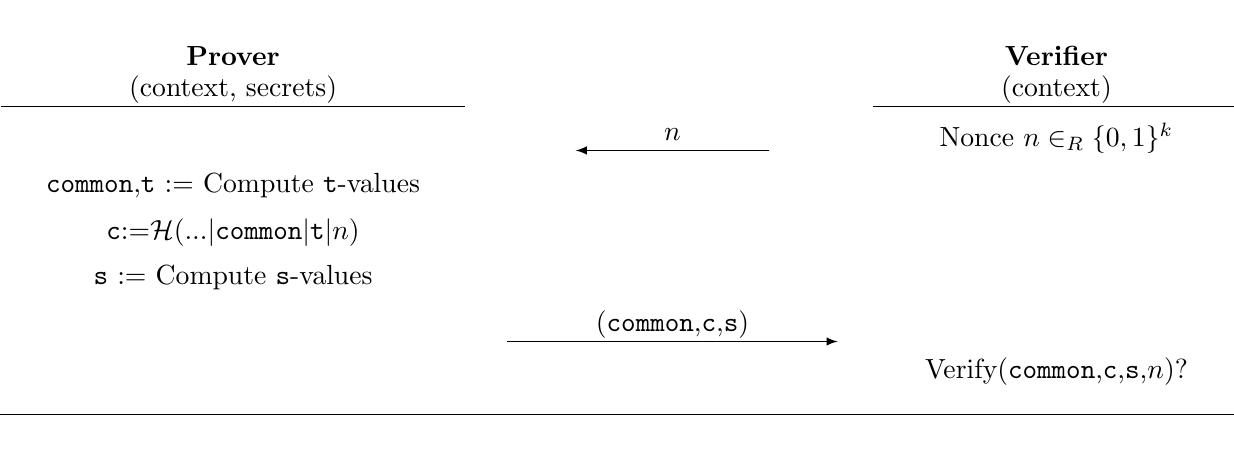
\begin{tikzpicture}
	\matrix (m)[matrix of nodes, column  sep=2cm,row  sep=1mm, nodes={draw=none, anchor=center,text depth=0pt} ]{
		\textbf{Prover} & & \textbf{Verifier}\\[-2mm]
		(context, secrets) & & (context)\\%[-4mm]
		& $n$ & Nonce $n \in_R \{0,1\}^{k}$ \\
		\texttt{common},\texttt{t} := Compute \texttt{t}-values  & & \\%[-8mm]
		\texttt{c}:=$\mathcal{H}$(...$\mid$\texttt{common}$\mid$\texttt{t}$\mid$$n$) & & \\
		\texttt{s} := Compute \texttt{s}-values & & \\
		& (\texttt{common},\texttt{c},\texttt{s}) & \\%[2.5mm]
		& & Verify(\texttt{common},\texttt{c},\texttt{s},$n$)? \\
		\hfil & \hfil & \hfil \\
	};
	
	\draw[shorten <=-1.5cm,shorten >=-1.5cm] (m-2-1.south east)--(m-2-1.south west);
	\draw[shorten <=-1.5cm,shorten >=-1.5cm] (m-2-3.south east)--(m-2-3.south west);
	\draw[shorten <=-1cm,shorten >=-1cm,-latex] (m-3-2.south east)--(m-3-2.south west);
	\draw[shorten <=-1cm,shorten >=-1cm,-latex] (m-7-2.south west)--(m-7-2.south east);
	\draw[shorten <=-3cm,shorten >=-2.5cm] (m-9-1.south west)--(m-9-3.south east);
	\end{tikzpicture}
\end{document}